\documentclass[runningheads]{llncs}
\usepackage{amssymb,booktabs,graphicx,xcolor,hyperref,array}
\usepackage{float}
\usepackage{placeins}
\usepackage{tikz}
\usetikzlibrary{arrows.meta,positioning,fit,calc,backgrounds}
\usepackage{enumitem}
\setlist{nosep,leftmargin=2em}
\graphicspath{{figures/}}
\hypersetup{colorlinks=true,linkcolor=blue,urlcolor=blue,citecolor=blue,
  hypertexnames=false}
\renewcommand{\topfraction}{0.92}
\renewcommand{\bottomfraction}{0.88}
\renewcommand{\textfraction}{0.08}
\renewcommand{\floatpagefraction}{0.72}
\setlength{\textfloatsep}{12pt plus 3pt minus 3pt}
\setlength{\floatsep}{10pt plus 3pt minus 3pt}
\makeatletter
\setlength{\@fptop}{0pt}
\setlength{\@fpsep}{12pt}
\setlength{\@fpbot}{0pt plus 1fil}
\makeatother
\setlength{\emergencystretch}{2em}

\newcommand{\method}{M1}
\newcommand{\full}{FullSchema}
\newcommand{\schemarag}{SchemaRAG}

\title{Budget-Aware Dynamic Schema Selection for Efficient LLM-Based Information Extraction Pipeline}
\titlerunning{Budget-Aware Dynamic Schema Selection}
\author{Hongjian Hu\inst{1} \and Letong Wang\inst{1} \and Yuanhai Lv\inst{2}
  \and Wanqing Zhao\inst{1} \and Shaobo Zhang\inst{1} \and Jinye Peng\inst{1}}
\authorrunning{Hu, H. et al.}
\institute{School of Information Science and Technology,\\
  Northwest University, Xi'an 710127, China
  \and Information Network Center,\\
  Xi'an University of Posts \& Telecommunications}

\begin{document}
\catcode`\`=\active
\def`#1`{\texttt{\detokenize{#1}}}
\maketitle

\begin{abstract}
\begin{sloppypar}
 Repeatedly transmitting Schema fields irrelevant to individual records increases the token workload of LLM information-extraction pipelines. We treat record-level Schema construction as pre-call semantic data pre-processing and present a budget-aware method trained from modest \full{} model-assisted silver supervision on museum records. A local sparse model predicts field presence and output length, while a 0--1 knapsack combines utility, estimated cost, and mandatory-field constraints to shape each request. On 500 frozen model-assisted evaluation-reference records, the deployed $n=100$, `budget-200` configuration covers 83.07\% of non-empty reference fields, with 16.93\% selection-stage omission. In a six-block paired benchmark with 2,000 records per run, it reduces mean LLM-token workload by 38.4\% and measured online pipeline time by 56.2\% relative to \full{}, while increasing effective throughput from 7.62 to 17.39 records/s. At a similar LLM-token workload, a fixed Top-$k$ embedding-retrieval adaptation has higher pipeline time and tail latency when query embedding is included. These results establish a bounded pipeline efficiency--completeness trade-off, not factual-quality equivalence, ranking optimality, zero-shot transfer, or production-scale scalability.
\end{sloppypar}
\end{abstract}

\keywords{Data pre-processing \and Schema selection \and Information extraction pipelines \and Dynamic Schema \and Large language models \and Field-load shaping \and Online throughput}

\section{Introduction}

LLM-based information extraction assembles raw records, instructions, and target Schemas before each model call. Repeatedly transmitting a fixed Schema with irrelevant fields increases token workload and can lengthen the end-to-end pipeline. Pre-call data preparation should therefore control both raw-input representation and request-level field load.

 Museum records provide a concrete setting: they share cataloguing conventions and recurring patterns but vary in information density and extractable fields. Existing structured-extraction and retrieval approaches can populate a supplied Schema or retrieve fields, but do not directly resolve the completeness--efficiency trade-off in pre-call record-level selection. Without large-scale human field annotations, modest \full{} model-assisted supervision may predict relevant fields for subsequent records from the same operating distribution. We ask whether semantic Schema pre-processing can reduce pipeline load while retaining fields in a separate model-assisted reference.

 We formulate pre-processing as budget-aware optimization. Sparse textual models predict field presence and output length; a 0--1 knapsack then constructs a dynamic Schema under estimated costs and mandatory-field constraints. The study contributes an auditable load-shaping framework, a completeness analysis, and a paired end-to-end comparison with \full{} and a fixed Top-$k$ embedding-retrieval adaptation. We report makespan, throughput, queue waiting, tail latency, success rate, and LLM-token workload under explicit concurrency and queue settings. The budget is estimated field-cost capacity, not an API-token or monetary limit, and the single-process evaluation does not establish distributed or production-scale performance.

\section{Related Work}

Relevant work spans several directions around structured extraction and flexible
context. UIE~\cite{uie}, InstructUIE~\cite{instructuie}, ChatSchema~\cite{chatschema},
and instruction-tuned LLMs such as InstructGPT~\cite{instructgpt} perform
extraction under predefined structures or instructions. GoLLIE~\cite{gollie} and
GLiNER~\cite{gliner} introduce guideline-conditioned or inference-time
flexibility. These approaches make extraction more general or controllable, but
do not themselves formulate record-level selection from a fixed candidate field
set under an explicit capacity constraint.

Retrieval and efficiency work reduces context or inference cost in different
ways. SchemaRAG~\cite{schemarag} and MetaRetriever~\cite{metaretriever} retrieve
task- or instance-relevant Schema information; SRSPSQL~\cite{srspsql} prunes
database schemas for Text-to-SQL, and context-aware prompt compression
~\cite{cpc} removes prompt sentences. IAPO~\cite{iapo}, LLMLingua
~\cite{llmlingua}, FrugalGPT~\cite{frugalgpt}, and Doctopus~\cite{doctopus}
optimize prompts, models, or execution plans. These directions reduce context or
cost, but do not combine an estimated field-cost capacity, mandatory-field
constraints, and a field-selection completeness analysis for a fixed candidate
Schema.

This work treats that selection as semantic pre-processing before each LLM call. From a fixed
18-field Schema, a lightweight local predictor estimates field presence and
output length; an estimated field-cost capacity and mandatory-field constraints
then determine the record-level subset. PARSE~\cite{parse}, Schema-adaptable
Knowledge Graph Construction~\cite{adakgc}, DSE-RE~\cite{dsere}, and schema-free
IE~\cite{schemafree} instead adapt, evolve, or generate Schemas. Our evaluation
combines model-assisted field-selection completeness with measured online
pipeline cost, without claiming factual-quality equivalence or Schema evolution.
The tested \schemarag{} configuration is a fixed Top-$k$ embedding-retrieval
adaptation based on its public description, not an official implementation or a
general conclusion about SchemaRAG. PagedAttention~\cite{pagedattention} is
orthogonal because it addresses serving-memory management; Huang et al.
~\cite{huang2023} and CHAD-KG~\cite{chadkg} provide cultural-heritage
knowledge-representation context rather than direct Schema-selection baselines.

\section{Method}

\subsection{Pre-call Schema Pre-processing and Problem Formulation}

Let $r$ denote a raw record, $F$ the candidate-field set, and $S_r\subseteq F$ the selected fields. For field $f$, the selector predicts a presence score $p(r,f)$ and an output-token count $\hat{o}(r,f)$. The field-value weight $w_f$ is an auditable task heuristic, not a weight learned as optimal from the present data, and $d_f$ is the field-definition cost. Dynamic selection is written as

\begin{equation}
 u(r,f)=p(r,f)w_f,
 \qquad c(r,f)=d_f+\hat{o}(r,f),
 \label{eq:utility-cost}
\end{equation}
\begin{equation}
 \max_{S_r}\sum_{f\in S_r}u(r,f),
  \quad \mathrm{s.t.}\quad \sum_{f\in S_r}c(r,f)\leq B.
\end{equation}

Here $B$ is the estimated field-cost capacity for the selection stage, not an end-to-end token or monetary-cost limit for the LLM call. Final tokens also include raw text, fixed Prompt, actual output, and retry consumption.

As shown in Fig.~\ref{fig:overall-framework}, the offline stage trains \method{} from \full{} silver labels. The online pre-processing stage serializes each record, predicts and selects fields under the budget, and constructs a dynamic Schema before the downstream LLM call and result write.

\begin{figure}[!ht]
\centering
\resizebox{\linewidth}{!}{%
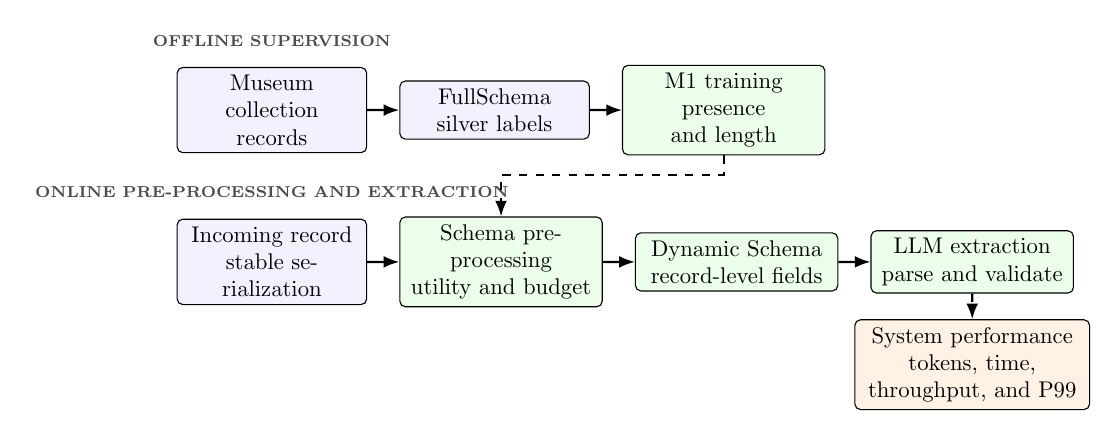
\begin{tikzpicture}[scale=0.82,transform shape,node distance=4mm and 5mm,
 data/.style={draw, rounded corners=2pt, align=center, minimum height=7mm, text width=27mm, fill=blue!5},
 process/.style={draw, rounded corners=2pt, align=center, minimum height=7mm, text width=29mm, fill=green!8},
 eval/.style={draw, rounded corners=2pt, align=center, minimum height=7mm, text width=34mm, fill=orange!10},
 stage/.style={font=\bfseries\scriptsize, text=black!70},
 arrow/.style={-{Latex[length=2mm]}, thick},
 dependency/.style={-{Latex[length=2mm]}, thick, dashed},
 evalarrow/.style={-{Latex[length=2mm]}, thick, dashed}]
\node[stage] (offline-title) {OFFLINE SUPERVISION};
\node[data, below=2mm of offline-title] (raw) {Museum collection\\records};
\node[data, right=of raw] (silver) {\full{}\\silver labels};
\node[process, right=of silver] (train) {\method{} training\\presence and length};
\draw[arrow] (raw) -- (silver);
\draw[arrow] (silver) -- (train);
\node[stage, below=4mm of raw] (online-title) {ONLINE PRE-PROCESSING AND EXTRACTION};
\node[data, below=2mm of online-title] (record) {Incoming record\\stable serialization};
\node[process, right=of record] (select) {Schema pre-processing\\utility and budget};
\node[process, right=of select] (schema) {Dynamic Schema\\record-level fields};
\node[process, right=of schema] (llm) {LLM extraction\\parse and validate};
\draw[dependency] (train.south) -- ++(0,-3mm) -| (select.north);
\draw[arrow] (record) -- (select);
\draw[arrow] (select) -- (schema);
\draw[arrow] (schema) -- (llm);
\node[eval, below=4mm of llm] (performance) {System performance\\tokens, time, throughput, and P99};
\draw[evalarrow] (llm.south) -- (performance.north);
\end{tikzpicture}%
}
\caption{Overall study design. Raw records construct \full{} silver-label supervision for \method{} training. The online path applies semantic Schema pre-processing before downstream LLM extraction. Evaluation reports model-assisted reference-field coverage and end-to-end pipeline performance; the reference is not independent human factual Gold.}\label{fig:overall-framework}
\end{figure}

\subsection{Data Representation and Silver Supervision}

The museum collection database contains 6,763 paired raw records and \full{} model-assisted extractions, split by record identifier into 5,410 training, 677 validation, and 676 test records. We consider 18 predefined target fields rather than arbitrary JSON keys; record identifiers are used only for pairing and dataset splitting. Record-type proportions in the performance workload differ from the source database by at most about 1.4 percentage points, and raw records usually contain only five non-empty fields; the results therefore do not claim coverage of all source distributions. A character 3-gram Jaccard scan (threshold 0.6) found 1,101 near-duplicate pairs and 111 clusters with a maximum size of 50; these structures and the 132 type--period proxy groups were retained to reflect the target distribution, without claiming independent generalization across templates or sources.

 The candidate Schema contains the same 18 fields. `name` and `category` are mandatory, `desc` uses a constant presence prediction, and the selector chooses the remaining fields per record. Several long-tail fields have silver non-empty rates below 2\%. Field weights are auditable task settings rather than learned optimal weights; complete definitions are provided in the repository. \full{} uses all fields, whereas the dynamic Schema selects a subset $S_r\subseteq F$.

The paired \full{} extractions provide model-assisted silver supervision, not human ground truth: a non-empty output for field $f$ gives `present=1`, and the `cl100k_base` token count of a non-empty value gives the length label. They are distinct from the separately generated 500-record evaluation reference; neither source verifies factual truth. \method{} therefore learns \full{} output behavior rather than independently verified facts.

\subsection{Lightweight Field-Presence and Length Prediction}

Raw JSON keys, values, and description text are stably serialized into a record-level text representation (`record_text`). The label $y_f(r)$ indicates whether the \full{} silver output for field $f$ is non-empty; the encoded length of a non-empty value supplies output-length supervision. Training, validation, and test sets are separated by record identifier, and validation is used only for threshold calibration. Each field uses an independent balanced logistic-regression classifier. The length branch fits $\log(1+o_f(r))$ and falls back to the median when positive examples are insufficient.

\method{} concatenates character-level and word-level TF--IDF features and outputs $p(r,f)$ and $\hat{o}(r,f)$; the character model is used only as a baseline. \textsc{M2} separately trains the two feature types and linearly fuses their probabilities, solely as an offline ablation. The vocabulary is fitted only on the training subset. Training sizes are $n\in\{50,100,250,500,1000,2500,5410\}$, using nested prefixes and seeds 42--46. `name`, `category`, and `desc` use constant predictions; insufficient positive examples for long-tail fields limit macro-averaged performance.

\begin{sloppypar}
\setlength{\emergencystretch}{4em}
 In a test replay of 100 startup samples, the character baseline achieved macro/micro Presence F1 and length MAE of $0.5187/0.9126/4.8046$. The corresponding values were $0.5088/0.9343/4.7615$ for \method{} and $0.5083/0.9341/4.7615$ for \textsc{M2}. \method{} provided only slight improvements in micro averaging and length error, while \textsc{M2} provided no additional benefit. Detailed per-field results and intervals from 35 offline runs are provided in the repository.
\end{sloppypar}

\subsection{Budgeted Record-Level Schema Pre-processing}

\begin{sloppypar}
Online, \method{} does not generate field values. The predictions are used with the mandatory-field constraint and a 0--1 knapsack to form $S_r$. Actual tokens are recorded from API calls.
\end{sloppypar}

\begin{figure}[htbp]
\centering
\includegraphics[width=\linewidth]{figures/m1_dynamic_selection_schematic.pdf}
\caption{M1-based Schema pre-processing. FullSchema silver labels
supervise offline training. Online presence and length estimates,
field weights, and estimated costs drive budgeted field selection.
M1 selects fields, not values; actual tokens are measured downstream.}
\label{fig:m1-selection}
\end{figure}

\section{Experiments}
\subsection{Experimental Setup}
\subsubsection{Compared Strategies and Controls}

Table~\ref{tab:strategies} distinguishes full-Schema, Prompt-only, dynamic-budget, and external-retrieval strategies.

\begin{table}[htbp]
\centering\scriptsize\renewcommand{\arraystretch}{0.88}
\caption{Inputs, selection mechanisms, and comparison roles of extraction strategies.}
\label{tab:strategies}
\resizebox{\linewidth}{!}{%
\begin{tabular}{>{\raggedright\arraybackslash}p{2.2cm}>{\raggedright\arraybackslash}p{3.3cm}>{\raggedright\arraybackslash}p{5.5cm}>{\raggedright\arraybackslash}p{3.4cm}}
\toprule
Strategy & Input fields & Field-selection or prompt mechanism & Comparison role\\
\midrule
`full` & All 18 fields & No pruning; base extraction prompt & Full-Schema baseline\\
`prompt-null` & All 18 fields & Output `null` without reliable evidence & Strict prompt-only baseline\\
`prompt-omit` & All 18 fields & Permit omitted fields without reliable evidence & Prompt-only output control\\
`budget-200/400` & Record-level field subset & \method{} prediction followed by a capacity-specific 0--1 knapsack & Dynamic strategy\\
`lambda` & Record-level field subset & \method{} prediction followed by a net-utility threshold & No-hard-budget control\\
`SchemaRAG k=8` & Top-$k$ field subset & Cosine ranking of query and field vectors & SchemaRAG-inspired efficiency reference\\
\bottomrule
\end{tabular}%
}
\end{table}

 `budget-200/400` retains mandatory fields and solves a 0--1 knapsack; the no-hard-budget control uses $u(r,f)-0.003c(r,f)$. The main experiment uses six balanced blocks, each running clean `full`, n=100 M1 `budget-200`, and \schemarag{} $k=8$ on the same frozen input order. Other online strategies run once, and additional offline diagnostics are provided in the repository.

Estimated field costs are used only for pre-call decisions:
\begin{equation}
 \widehat{C}_{field}(r,f)=C_{schema}(f)+\widehat{C}_{output}(r,f).
\end{equation}
Here $C_{schema}(f)$ counts the field name and definition in `cl100k_base` tokens, and $\widehat{C}_{output}(r,f)$ is \method{}'s non-negative, truncated prediction of output length. This is not the actual API cost. The API records `input_tokens`, `output_tokens`, and `total_tokens` after the call, including retry overhead. Raw-record input and the fixed Prompt are usually sent regardless of field selection; they are excluded from the field-combination budget but included in online LLM token statistics.

\subsubsection{Tested Embedding-Retrieval Adaptation}

\schemarag{} is implemented as a SchemaRAG-inspired semantic field-selection reference for the same downstream LLM extraction pipeline. It does not use \method{} predictions or budget knapsack selection; instead, it ranks candidate fields by semantic similarity between the record and field descriptions. The candidate Schema in this study contains 18 fields, so this comparison evaluates field-load reduction in a compact JSON extraction setting rather than the large-Schema regime targeted by the original work.

\paragraph{Retrieval Representation and Field Ranking.}

Field-name and field-definition vectors are weighted 0.5/0.5 and normalized. The serialized JSON record and a fixed instruction form the single online query, and Top-8 fields are selected by cosine similarity. Thus, $k=8$ retains 44.4\% of the 18-field candidate Schema, closely matching the 7--9 fields usually selected by `budget-200`. The original work instead targets much larger schemas, so its reported scale and $k$ are not directly comparable with ours. This adaptation uses only field-name and field-definition retrieval: it does not include optional example retrieval, in-context examples, text segmentation, or reranking. Field vectors are cached, while query embedding is included in pipeline time. The adaptation used Qwen3-Embedding-0.6B~\cite{zhang2025qwen3embedding}, batch size 32, a 60-s timeout, and 1024-dimensional vectors. It is an external efficiency reference, not a complete reproduction of the original implementation. The embedding service does not return usage information, and its token consumption and server-side version cannot be reconstructed from the local archive.

\subsubsection{End-to-End Pipeline Execution and Metrics}

The implementation is a single-process asynchronous pipeline with a Producer, multiple Consumers, and a bounded queue. Schema pre-processing precedes request submission. Concurrency `c` sets the number of Consumers and `q` the queue capacity; a full queue blocks the Producer and creates backpressure. Tasks are built incrementally in input order, support checkpointed resumption by method and configuration hash, and retain errors after at most two retries.

We define makespan as the interval $t_{finish}-t_{start}$ and effective throughput as $N_{success}$ divided by makespan. The `pipeline_ms` interval covers online record reading, field prediction and selection, Prompt construction, enqueueing, LLM or embedding requests, retries, and result writing; each task stores Prompt, Schema, selector and method configuration hashes, selected fields, predicted and actual tokens, planning or retrieval time, latency, queue waiting, and error state.

The measured interval excludes startup-sample generation, silver-label construction, offline training, and model or vectorizer loading. Results cover the online pipeline, not full-lifecycle costs; `budget-200` is neither a 200-token limit nor a global optimum. Execution remains single-process without cross-process or cross-node scheduling, on museum records rather than HPC simulation outputs.

\subsubsection{Evaluation Reference and Metrics}

 Let $G_r$ be the non-empty fields in the model-assisted evaluation reference and $S_r$ the selected set. Unlike the \full{} silver labels used to train M1, this reference was generated at temperature 0 using only the raw record, with JSON null required when evidence was unreliable; it is not human factual Gold. We define coverage as $\mathrm{Cov}(r)=|S_r\cap G_r|/|G_r|$ and omission as $\mathrm{Miss}(r)=1-\mathrm{Cov}(r)$. This measures field entry into the target Schema, not downstream output or factual correctness. All quality results use the same 500 frozen reference records. The cross-institution holdout instead uses an external evidence silver reference (\texttt{agent-evidence-reference-v2}) generated by an LLM-free script from raw-record-supported fields; it is independent of the evaluated model but conservative.

\subsubsection{Workload and Experimental Conditions}

The performance workload contains 2,000 records from training and validation sets and does not overlap the test set, but overlaps \method{}'s development distribution and threshold calibration and is therefore not an independent generalization test. The same snapshot was used in six balanced blocks, each running clean `full`, n=100 M1 `budget-200`, and \schemarag{} $k=8$ in a different serial order. The three methods used the same served Qwen3-8B-AWQ~\cite{yang2025qwen3} model service, Prompt, Schema, $c=16,q=16$, and explicit extra-field allowance; extra fields were retained for audit. Statistics use the six blocks as units, not the 2,000 records as independent replicates.

For cross-institution validation, we removed non-semantic provenance fields, including source URLs, from 500 ID-disjoint records of a second museum collection. One \full{} run supplied silver labels for 100 training and 50 validation records. M1 was retrained on these subsets; both budgets were evaluated on the 350 held-out records against the external evidence reference, not the \full{} training output.

\subsection{Experimental Results}
\subsubsection{Main Field-Selection Comparison}

\begin{table}[htbp]\centering\small
\caption{Field-selection completeness on 500 frozen model-assisted evaluation-reference records.}\label{tab:coverage}
\begin{tabular*}{\linewidth}{@{\extracolsep{\fill}}lccc@{}}\toprule
Method & Records & Reference-field coverage & Selection omission rate\\\midrule
full & 500 & 1.0000 & 0.00\%\\
budget-200 & 500 & 0.8307 & 16.93\%\\\bottomrule
\end{tabular*}\end{table}

The zero omission of `full` follows from sending every candidate field and does not imply factual correctness. `budget-200` retains 83.07\% of non-empty reference fields, with 16.93\% omitted at selection. This is a measurable load--completeness trade-off, not lossless pruning.

 On the same 500 records, we further compare six internal Schema strategies in Table~\ref{tab:eight}. After lower-casing, trimming, and removing whitespace, a field is positive when its reference or generated value is non-empty. Mean record F1 averages record-level presence F1 values; Micro-F1 aggregates field-level TP/FP/FN; Exact Value Recall is the fraction of reference-positive fields whose normalized generated value exactly matches the reference. These are output-agreement metrics, not evidence of factual quality or global optimality.

\begin{table}[htbp]
\centering
\scriptsize
\setlength{\tabcolsep}{2pt}
\caption{Output agreement, field coverage, and LLM tokens per record on 500 frozen records. Agreement is against the model-assisted reference, not factual Gold. `prompt-omit` was rerun; 23/500 raw responses with an unambiguous missing JSON value were repaired offline as `null` without new model calls, so this row is not a timing comparator.}
\label{tab:eight}
\resizebox{\linewidth}{!}{%
\begin{tabular}{lccccc}
\toprule
Method & Mean record F1 & Micro-F1 & Exact Value Recall & Coverage & Total tokens\\
\midrule
full & .7576 & .7364 & .6533 & 1.0000 & 539.19\\
prompt-null & .6192 & .5853 & .6579 & 1.0000 & 547.48\\
prompt-omit & .7492 & .7402 & .6026 & 1.0000 & 530.63\\
budget-200 & .7750 & .7771 & .6222 & .8307 & 380.95\\
budget-400 & .7743 & .7648 & .6628 & .9774 & 485.75\\
lambda=0.003 & .7812 & .7809 & .6401 & .9596 & 440.08\\
\bottomrule
\end{tabular}%
}
\end{table}

 Table~\ref{tab:eight} shows that full-field prompting is not an output-agreement ceiling against the development-collection reference, while prompt constraints alone do not eliminate extra fields. On the ID-disjoint cross-institution holdout, under the independent evidence reference the three methods fall in a narrow band (mean record F1 .490--.520; Micro-F1 .480--.520): `budget-200` has the highest Micro-F1 (.5203) and lowest tokens (370.06, 24.79\% below \full{}); `budget-400` has the highest record F1 (.5196) at 469.82 tokens (4.51\% below \full{}); \full{} is lowest with the most unsupported fields (mean 10.30 per record). Absolute agreement is low because the reference is conservative and the model small, so these values support only relative comparison, not absolute quality or zero-shot transfer.

\subsubsection{Selection-Strategy Ablation and Weight-Sensitivity Diagnostics}

 To separate fewer fields from a ranking mechanism, we compare selection strategies on 500 frozen model-assisted reference records using five \method{} training seeds under the same mandatory fields and budget. Table~\ref{tab:selection-ablation} reports selection-stage coverage; its 57.94\% weighted budget-200 result is a five-seed mean with record-wise field-count matching, whereas Table~\ref{tab:coverage} reports one deployed n=100 configuration. The values are therefore not interchangeable.

 Random Top-$k$ is substantially lower at both budgets, indicating that arbitrary field reduction does not preserve reference fields equally well. The current hand-weighted strategy is not consistently better than equal weighting, training frequency, or simple Top-$k$: after $\pm20\%$ multiplicative perturbations, coverage at budgets 200/400 was 57.51\% and 94.00\%, close to the original 57.94\% and 94.22\%, so no catastrophic decline occurred but unique or optimal weights are not established. The five-seed sensitivity intervals used the Student-$t$ distribution. Neither perturbation nor random Top-$k$ represents 100 independent model trainings.

\begin{table}[htbp]\centering\scriptsize
\caption{Selection-stage reference-field coverage (\%) on 500 frozen model-assisted reference records.}\label{tab:selection-ablation}
\begin{tabular*}{\linewidth}{@{\extracolsep{\fill}}crrrrrr@{}}\toprule
Budget & Weighted & Equal & Frequency & \method{} Top-$k$ & Static Top-$k$ & Random Top-$k$\\\midrule
200 & 57.94 & 61.23 & 60.88 & 65.55 & 65.55 & 46.03\\
400 & 94.22 & 93.16 & 95.06 & 94.68 & 95.97 & 60.86\\\bottomrule
\end{tabular*}\end{table}

\subsubsection{End-to-End Pipeline Comparison}

\begin{sloppypar}
 Across six paired blocks, `budget-200` reduced mean pipeline time by 147.556 s (95\% paired CI 144.747--150.364), mean LLM tokens per run by 684,031.8 (681,318--686,745), and increased effective throughput by 9.776 records/s (9.418--10.134) relative to clean `full`; mean blockwise E2E P95/P99 was lower by 2,822.8 ms (2,694.9--2,950.7) and 3,281.1 ms (2,665.4--3,896.8). The tested embedding-retrieval adaptation used a similar LLM-token load but increased mean pipeline time by 142.761 s and E2E P95/P99 by 18,788.4/46,371.1 ms; mean query-embedding time was 260.064 s per run. This is an efficiency comparison only, not evidence of equivalent field-selection completeness or output agreement. All 36,000 requests succeeded without retries. Extra-field auditing found 1/12,000 clean-full records, 0/12,000 budget records, and 557/12,000 retrieval-adaptation records with extra fields, with 1,099 occurrences. These fields were retained in `unexpected_fields` and did not change success counts. LLM tokens include input and output but exclude embedding; the intervals describe six run-level paired blocks, not other services or deployment conditions.
\end{sloppypar}

\begin{table}[t]\centering\scriptsize
\caption{Six-block means per 2,000-record run on the common development-distribution workload. Every method completed 12,000/12,000 pooled requests.}\label{tab:system}
\begin{tabular*}{\linewidth}{@{\extracolsep{\fill}}lcccc@{}}\toprule
Method & Mean time (s) & Mean throughput & LLM tokens/run & E2E P99 (ms)\\\midrule
clean full & 262.588 & 7.617 & 1,783,438 & 6,008.2\\
budget-200 & 115.033 & 17.393 & 1,099,406 & 2,727.1\\
SchemaRAG $k=8$ & 405.349 & 5.202 & 1,084,845 & 52,379.3\\\bottomrule
\end{tabular*}\end{table}

\begin{figure}[t]\centering
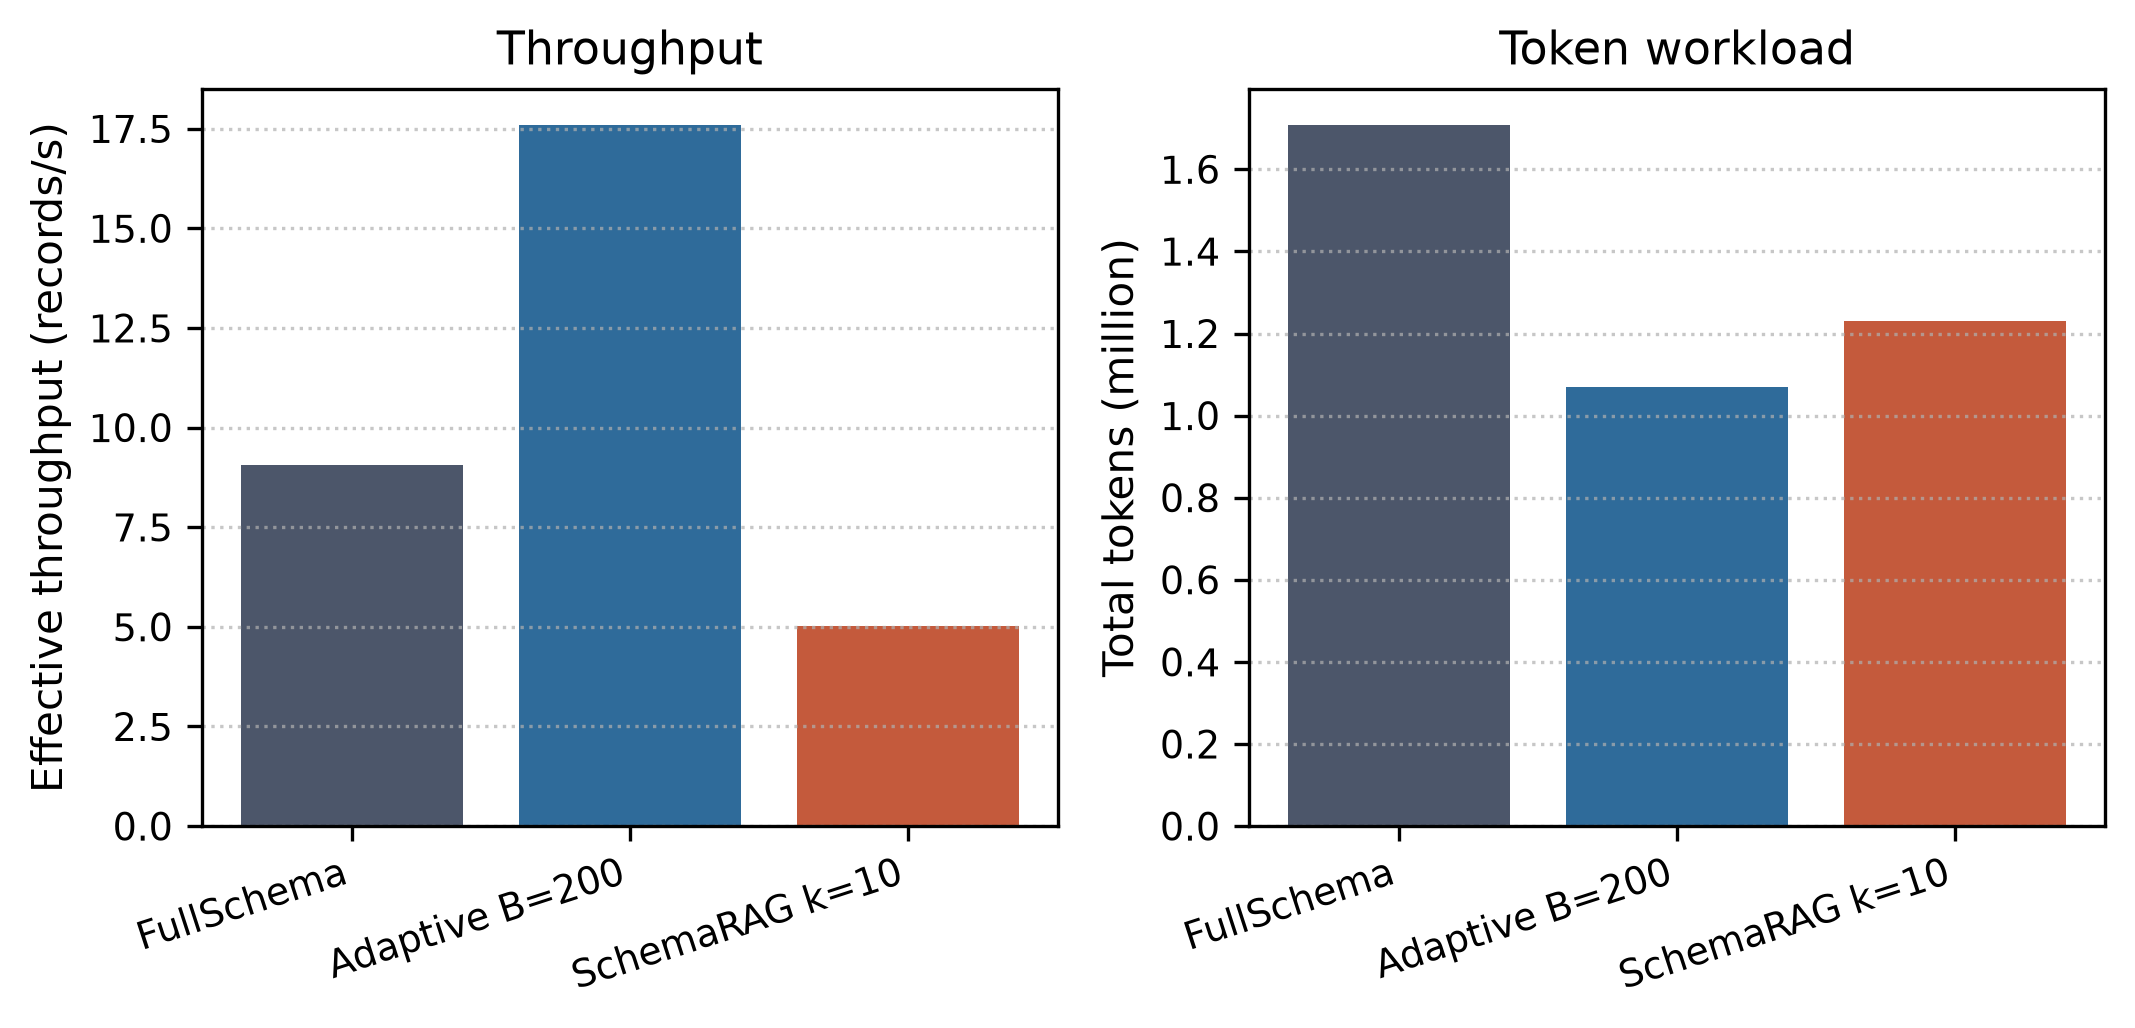
\includegraphics[width=.42\linewidth]{main_throughput_and_tokens.png}\hfill
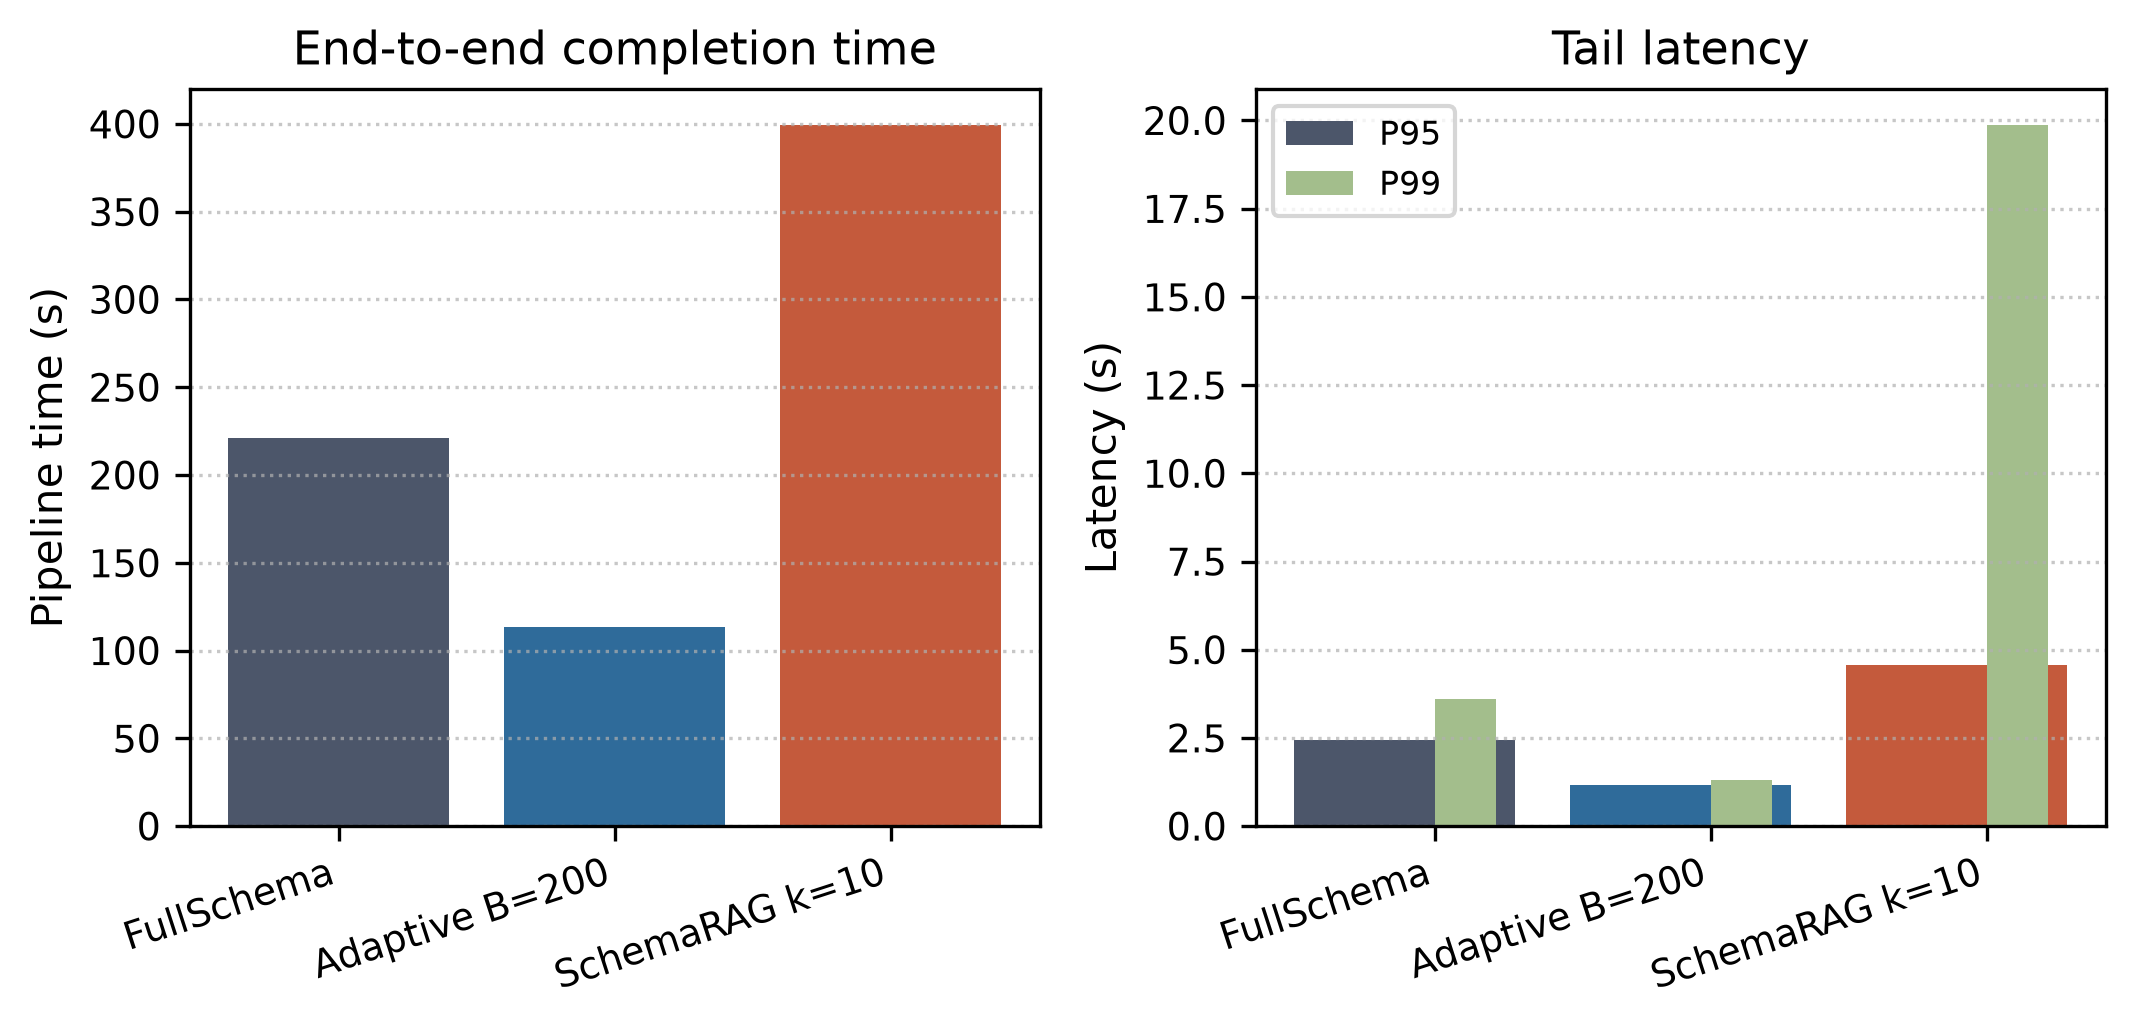
\includegraphics[width=.42\linewidth]{main_time_and_tail_latency.png}
\caption{Six-block mean online metrics per 2,000-record run, including effective throughput, LLM token workload, makespan, and blockwise record-level E2E P99. The comparison is limited to the stated service and concurrency configuration.}\label{fig:system-main}
\end{figure}

\FloatBarrier
\subsubsection{Initialization Cost and Deployment Boundary}

 Isolated training on 100 \method{} samples took $737.13\pm43.69$ ms; the model occupied 3.36 MB and cold loading took $178.26\pm14.43$ ms. A local planning batch of 100 records took 366.63 ms, while the independent stage measurement was $3.09\pm0.16$ ms per record and complete planning plus prediction and Prompt construction took approximately 6.2 ms per record; these measurements use different scopes. With $N_{\mathrm{BE}}=C_{\mathrm{startup}}/(T_{\mathrm{full}}-T_{\mathrm{budget}})$ and a measured online saving of 0.07351 s per record, break-even is approximately 2.43 records when charging only cold loading (0.17826 s), or 12.45 records when charging local training plus loading (0.91539 s) (Fig.~\ref{fig:init-cost}); token break-even is zero. \schemarag{} did not obtain a time benefit in the current range. These are scope-specific estimates, excluding startup-sample generation, silver preparation, environment startup, and cold-cache effects, not a monetary or full-lifecycle audit.

\begin{figure}[tb]\centering
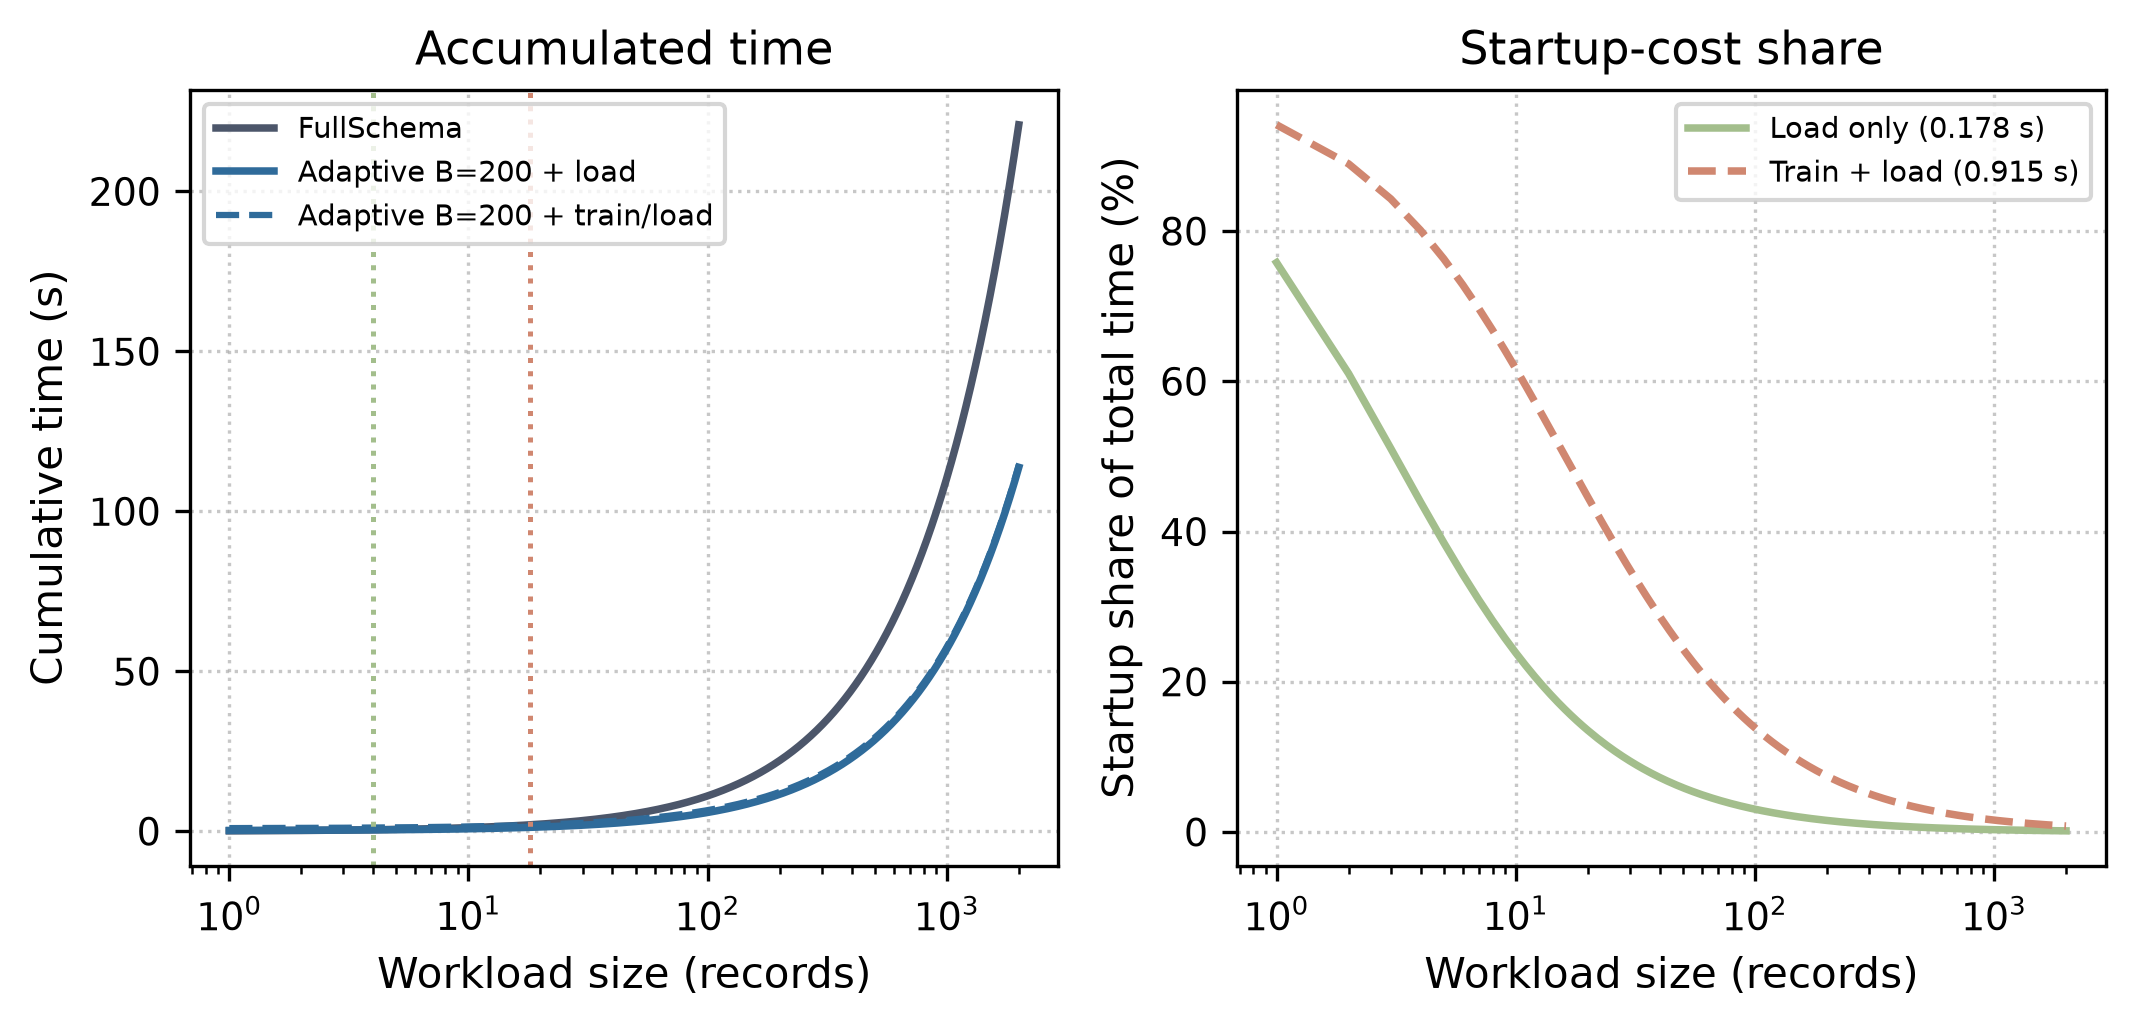
\includegraphics[width=.72\linewidth]{initialization_cost_sensitivity.png}
\caption{Initialization-cost sensitivity and the budget--full time break-even. The curve marks the one-time startup cost and the point where the dynamic-selection overhead is recovered.}\label{fig:init-cost}
\end{figure}

\subsubsection{Budget and Additional Baseline Analyses}

We scanned nine budget settings once under the same 2,000-record workload and $c=16,q=16$. The field ratio is selected fields divided by the 18 candidate fields, not reference-field coverage; tokens are the sum of actual LLM input and output, and the budget remains only a selection-stage capacity.

\begin{table}[htbp]\centering\scriptsize
\caption{Single-run online budget response on the 2,000-record frozen workload.}\label{tab:budget-response}
\begin{tabular*}{\linewidth}{@{\extracolsep{\fill}}rrrrrr@{}}\toprule
Budget & LLM Token/record & Fields/record & Fields/18 (\%) & P99 (ms) & Success (\%)\\\midrule
60 & 326.7 & 2.80 & 15.5 & 1240 & 100.00\\
100 & 404.0 & 4.15 & 23.1 & 993 & 100.00\\
150 & 482.4 & 5.90 & 32.8 & 1186 & 99.95\\
200 & 534.6 & 7.52 & 41.8 & 1445 & 100.00\\
300 & 627.4 & 10.13 & 56.3 & 1706 & 100.00\\
400 & 730.7 & 13.73 & 76.3 & 2818 & 100.00\\
600 & 856.1 & 18.00 & 100.0 & 3883 & 100.00\\
800 & 857.6 & 18.00 & 100.0 & 3870 & 100.00\\
1200 & 858.0 & 18.00 & 100.0 & 3915 & 100.00\\\bottomrule
\end{tabular*}\end{table}

\begin{figure}[htbp]\centering
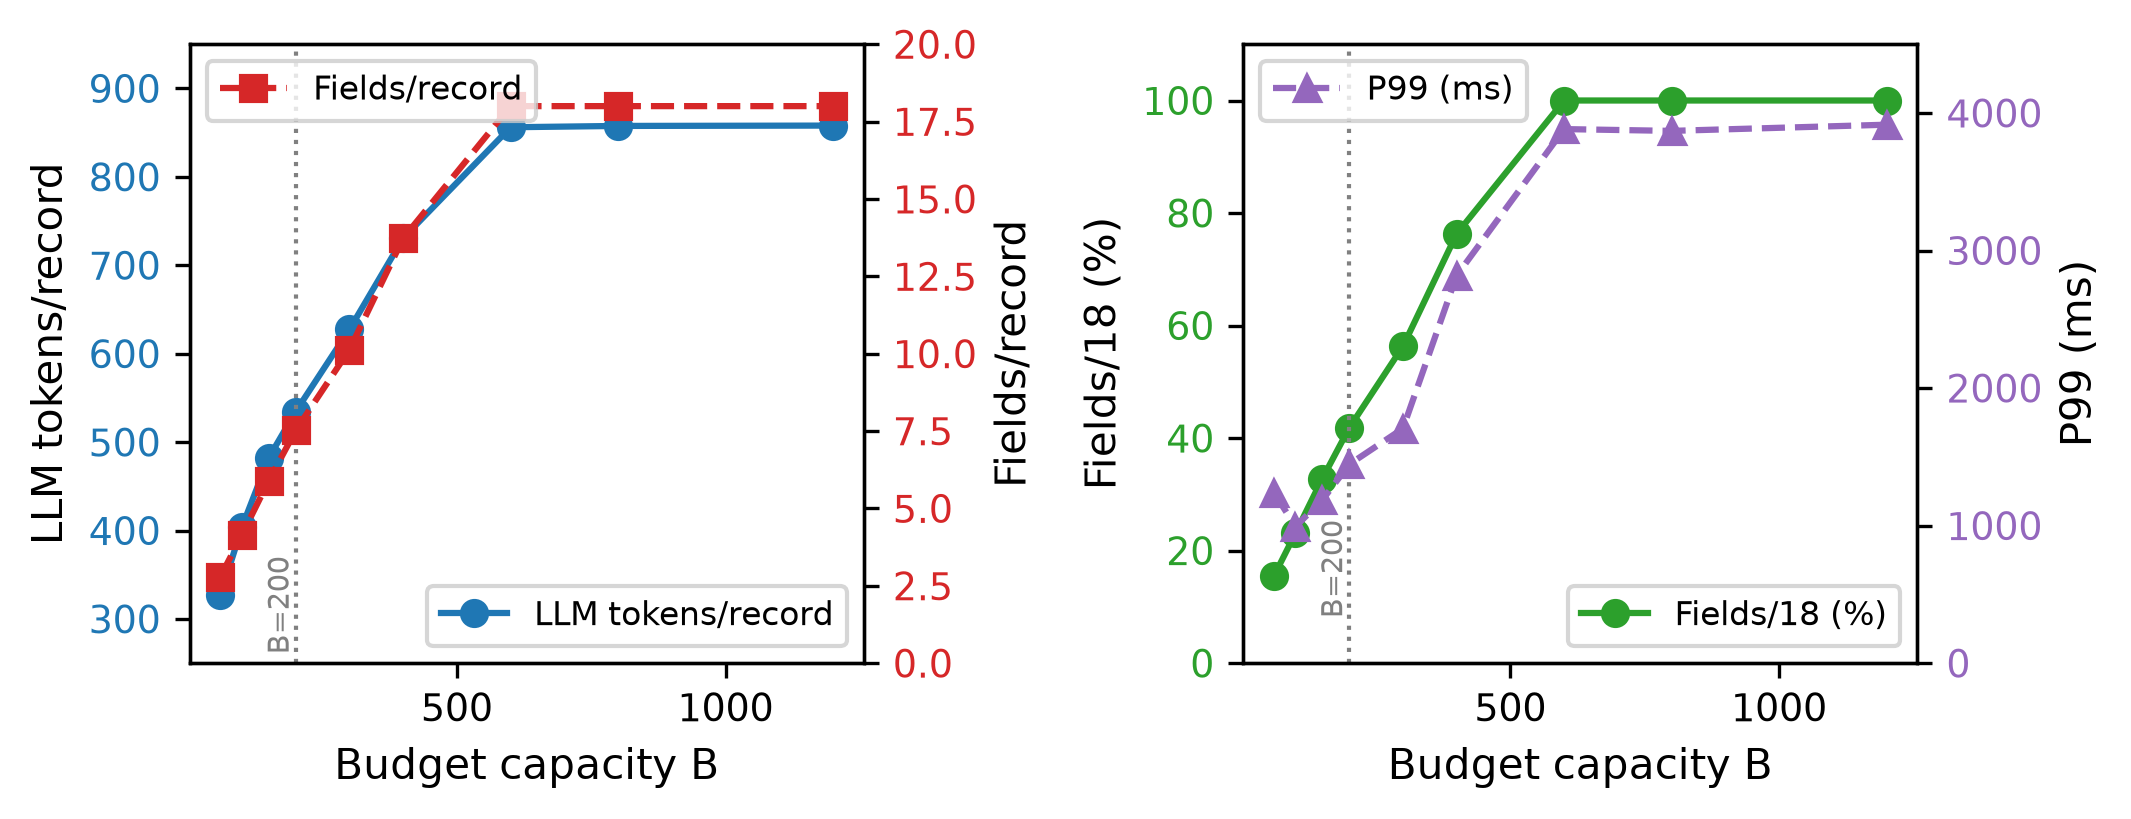
\includegraphics[width=.72\linewidth]{budget_response.png}
\caption{Online budget response on the 2,000-record frozen workload (single run each). Left: LLM tokens/record and fields/record; right: Fields/18 (\%) and P99; the dashed line marks $B=200$.}\label{fig:budget-response}
\end{figure}

Actual tokens and field counts generally increase with the budget and saturate near 600 units, when all 18 fields are selected. `budget-200` is therefore a low-to-intermediate operating point, not a global optimum; its 41.8\% field ratio does not measure reference-field completeness.

 In a single additional baseline run, LLM tokens per record for $\lambda=0.003$, prompt-omit, and prompt-null were 625.5/823.2/892.6, and P99 values were 3575/2542/3903 ms. Prompt-only controls still used all fields, indicating that token reduction mainly comes from reducing the number of fields; \method{}'s ranking advantage has not been established. Random/frequency Top-$k$ online results remain unavailable.

\subsubsection{Concurrency and Queue Sensitivity}

To separate the directional effects of concurrency and queue capacity, we scanned 500 records: with $c=16$ fixed, $q\in\{4,8,16,32,64\}$; with $q=16$ fixed, $c\in\{1,2,4,8,16,32\}$. Every point used `budget-200` and achieved 500/500 successes; the first $q=64$ run submitted only 182 records owing to a shell timeout and was replaced by a clean rerun of all 500. With $c=16$ fixed, throughput was 21.04, 21.31, 21.54, 20.20, and 21.01 records/s for the five queue sizes, while queue-wait P99 was 578, 758, 997, 1,908, and 3,265 ms. With $q=16$ fixed, throughput was 1.67, 3.34, 6.52, 11.80, 21.54, and 30.19 records/s for the six concurrency levels.

With fixed $c$, increasing $q$ mainly raises the queue-wait tail without a stable throughput gain. With fixed $q$, increasing $c$ improves throughput but high concurrency raises tail latency. This scan remains single-process and cannot establish production-scale scalability; it also shows that optimization should monitor time, success rate, and tail latency in addition to token minimization.

\subsection{Discussion}

Under the tested single-process configuration, `budget-200` reduced
LLM-token workload and makespan while increasing effective throughput.
Query-embedding overhead offset field-load savings in the tested
retrieval adaptation. Evaluation should therefore jointly consider
completeness, end-to-end time, throughput, success rate, and tail latency.

The budget scan supports capacity-based load control and saturation,
not optimal ranking, field importance, or factual-quality equivalence.
Neither the approximate field-count baseline nor the offline ablation
establishes a stable advantage for M1's weighted knapsack.

The references are non-human, and the main workload follows the
development distribution. The ID-disjoint cross-institution holdout
requires 100 same-cohort FullSchema silver labels; its conservative
reference permits only relative comparisons, not claims of zero-shot
or temporal transfer. The 18-field retrieval experiment does not
support general conclusions about \schemarag{}. Distributed execution,
larger scales, memory and lifecycle costs, and HPC workloads remain
unevaluated. Human-validated evaluation on unseen workloads is needed.
Code, frozen artifacts, configurations, scripts, and the scoped
`prompt-omit` repair procedure are available in the repository.

\section{Conclusion}

We presented budget-aware dynamic Schema pre-processing trained from
FullSchema model-assisted silver labels. On the 2,000-record museum
workload with a single-process Runner ($c=16,q=16$), M1 `budget-200`
reduced LLM-token workload and pipeline time while increasing
throughput. Selection coverage on 500 separate model-assisted reference
records was 83.07\%, with 16.93\% omitted.

After retraining on 100 same-cohort silver labels, `budget-200/400`
reduced cross-institution-holdout LLM tokens by 24.79\%/4.51\%,
without underperforming FullSchema under the independent reference.
These results support an efficiency--completeness trade-off, not
lossless pruning, factual-quality equivalence, zero-shot transfer,
or distributed, HPC, or production-scale scalability.

\section{Acknowledgments}
This research was supported by the National Natural Science
Foundation of China (Grant Nos. 62273275 and 62572393) and
the Key Research and Development Plan of Shaanxi Province
(Grant No. 2025GH-YBXM-018).

\bibliographystyle{splncs04}
\bibliography{references}
\end{document}
